\chapter{Clinical Relevance of CT Habitats}\label{clinical-relevance-of-ct-habitats}\label{ch:8}

In Chapter~\ref{ch:7}, we developed an mpMRI-anchored CT habitat model that
segments colorectal liver metastases into three biologically meaningful
compartments: avascular core, cellular-perfused viable tumor, and
vascular rim. Histopathological validation confirmed that this spatial
architecture reflects genuine tumor biology. In this chapter, we address
the central follow-up question: Do these biologically-grounded habitats
provide clinical value beyond standard imaging biomarkers?

\textbf{Contributions:}

\begin{itemize}
\item
  We assess whether habitat-derived metrics predict survival
  independently of tumor volume across two clinical contexts: resectable
  disease treated with curative-intent surgery (TCIA, n=189) and
  unresectable disease treated with palliative systemic therapy (VHIO,
  n=344).
\item
  We evaluate how treatment context modifies prognostic value, testing
  whether habitat metrics are informative after neoadjuvant chemotherapy
  (TCIA) and with anti-angiogenic therapy (VHIO).
\item
  We test whether prognostic signal concentrates at specific spatial
  locations, comparing rim, core, and whole-tumor metrics.
\item
  We explore whether longitudinal habitat changes during treatment
  capture response biology that RECIST classification misses, focusing
  on the ambiguous stable disease category.
\end{itemize}

\begin{quote}
The work presented in Chapters 7 and 8 forms the basis of a manuscript
currently in preparation.
\end{quote}

\section{Rationale}\label{rationale-2}

Tumor volume is the dominant imaging biomarker in oncology. Together
with anatomical location, it determines resectability and guides the
choice between curative surgery and palliative systemic therapy. RECIST
criteria \citep{eisenhauerNewResponseEvaluation2009}, which inform treatment decisions
across solid tumors, define response and progression primarily through
size change. This framework works reasonably well when tumors shrink or
grow substantially ---but there are moments during treatment when
changes in size are not informative

The limitation is not volume itself but what volume ignores: the
internal composition of the tumor. A 30 cm³ metastasis that is 80\%
necrotic differs fundamentally from one that is 80\% viable tumor---yet
both receive identical volumetric assessment. This matters for two
clinical problems. First, response assessment: a tumor that neither
shrinks nor grows might be genuinely controlled by treatment, or it
might be slowly progressing. Survival outcomes among volumetrically
similar patients vary widely, yet current imaging cannot distinguish
these scenarios. Second, treatment selection: many patients do not
respond as expected to first-line therapy, and we lack imaging tools to
predict who will benefit from which regimen. Both problems---assessing
response and selecting treatment---could benefit from imaging biomarkers
that characterize tumor heterogeneity beyond size.

Habitat imaging offers a potential solution. By segmenting tumors into
spatially distinct subregions with different imaging phenotypes,
habitats capture the heterogeneity information that volume discards. In
Chapter 7, we established that CT habitats in colorectal liver
metastases reflect vascular architecture: an avascular compartment
representing necrotic or fibrotic tissue, a cellular-perfused
compartment representing viable tumor, and a vascular rim at the
tumor-liver interface. If these phenotypes have prognostic relevance,
habitat-derived metrics should predict survival independently of
volume---and potentially discriminate outcomes among volumetrically
similar patients.

This chapter tests these hypotheses across two cohorts with
complementary clinical contexts:

TCIA cohort (n=189, resectable disease): Patients underwent hepatic
resection with curative intent; 60\% received neoadjuvant chemotherapy.
We ask: Does neoadjuvant treatment alter habitat composition? Do
post-treatment habitat patterns predict survival? We hypothesize that
treatment remodels tumor composition in ways detectable by CT, and
that spatial heterogeneity at the invasive rim will carry prognostic
information beyond what volume provides.

VHIO cohort (n=344, unresectable disease): Patients received first-line
systemic therapy---chemotherapy alone, chemotherapy plus bevacizumab, or
chemotherapy plus targeted agents. We ask: Do baseline habitat metrics
predict survival? Does prognostic value depend on treatment type and
molecular context? We hypothesize that for cytotoxic chemotherapy, where
response manifests as tumor shrinkage, volume will dominate. For
anti-angiogenic therapy, where treatment slows growth without
necessarily shrinking tumors, spatial heterogeneity at the rim may
capture treatment-relevant biology that volume cannot.

A subset of VHIO patients (n=38) had paired baseline and follow-up
imaging, allowing us to ask a third question: Does the direction of
habitat change during treatment predict outcomes beyond what RECIST
categories provide? If rim heterogeneity captures treatment response,
then the direction of rim entropy change may differ systematically
between responders and progressors.

\section{Methods}\label{methods-2}

\subsection{Patient Cohorts}\label{patient-cohorts-2}

Two independent cohorts were analyzed (\Cref{fig:8.1}A, \Cref{tab:clinical_characteristics}). The TCIA cohort included
189 patients with resectable colorectal liver metastases from a publicly
available dataset. All patients underwent hepatic resection with
curative intent; 115 (60.8\%) received neoadjuvant chemotherapy prior to
surgery. CT imaging was acquired pre-surgery, representing
post-neoadjuvant status in treated patients and treatment-naive status
in untreated patients.

The VHIO cohort included 344 patients with unresectable metastatic
colorectal cancer treated at Vall d\textquotesingle Hebron Institute of
Oncology. All patients received first-line systemic therapy:
chemotherapy alone (n=122), chemotherapy plus bevacizumab (n=133), or
chemotherapy plus targeted therapy (n=69). CT imaging was acquired at
baseline (pre-treatment) for all patients; a subset of 38 patients had
paired follow-up imaging for longitudinal analysis. RAS mutation status
was available for 331 patients (96\%): 136 RAS wild-type, 195 RAS
mutant. Inclusion criteria and image preprocessing for both cohorts are
detailed in Section 5.1.

\subsection{Habitat Computation}\label{habitat-computation}

CT habitats were computed using the biologically-anchored model
developed in Chapter~\ref{ch:7} (Section 7.3.1). Briefly, six handcrafted
features were computed from contrast-enhanced CT (portal phase) and
clustered using a Gaussian mixture model (K=3) in two steps (hybrid mode
in the imaging habitats pipeline, see Section 5.2). The handcrafted
representation was selected over alternatives (raw HU, deep learning
features) based on its superior ability to separate biologically
distinct tissue compartments as measured by co-registered
multiparametric MRI.

This produced three habitats (\Cref{fig:8.1}B):
the avascular habitat (corresponding to necrotic-like or poorly perfused
tissue with low cellularity), the cellular-perfused habitat (highest
cellularity and perfusion, corresponding to viable tumor), and the
vascular habitat (moderate cellularity and high vascularity). The
vascular habitat may partly reflect partial volume effects at the
tumor-liver interface. The biologically-anchored approach ensured that
habitats captured cellular and vascular heterogeneity validated against
ground truth rather than arbitrary clusters.

\subsection{Habitat-Derived Quantitative Metrics}\label{habitat-derived-quantitative-metrics-1}

Quantitative metrics were derived at three spatial scales: whole tumor,
rim (outer 2mm), and core (tumor interior)
(\Cref{fig:8.1}C).

For each scale, we computed habitat proportions (fraction of voxels
assigned to each habitat) and Shannon entropy (diversity of habitat
composition). Higher entropy indicates a more heterogeneous mixture of
habitats; lower entropy indicates dominance by a single habitat. Tumor
volume was computed as the sum of tumor voxels multiplied by voxel
spacing. These metrics follow the definitions in Section 5.2.3. For
patients with multiple liver metastases, metrics were aggregated across
lesions using volume-weighted averaging, giving greater weight to larger
lesions.

\begin{figure}[htbp]
\centering
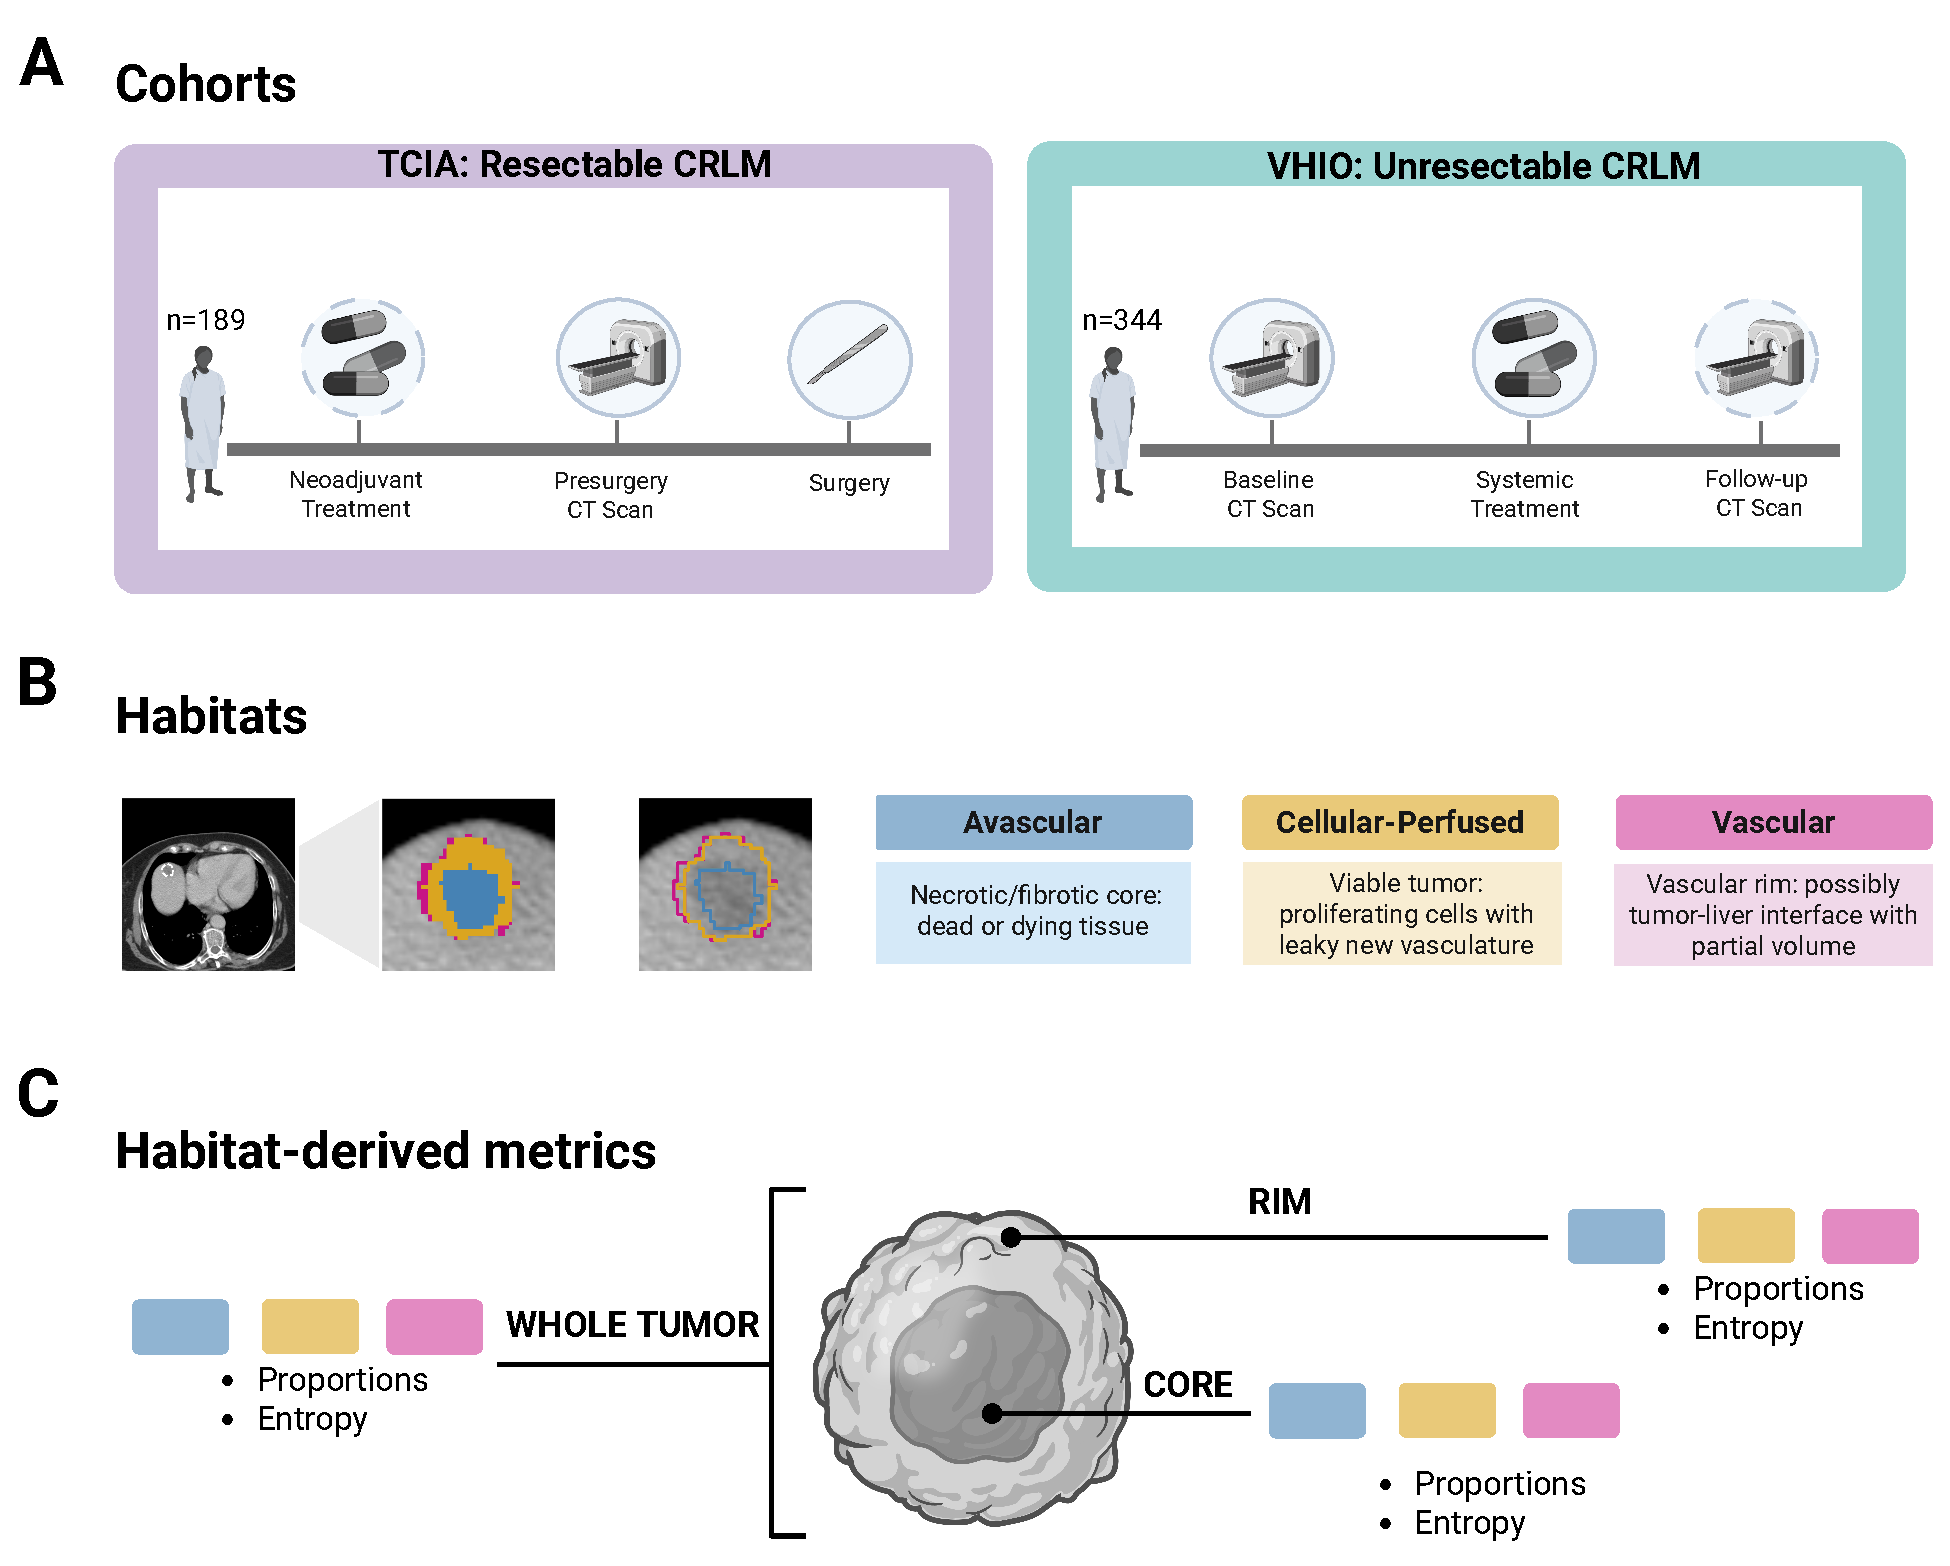
\includegraphics[width=0.95\textwidth]{fig_8_1.pdf}
\caption[Clinical validation study design]{Clinical validation study design.
\textbf{(A)} Two independent cohorts with distinct clinical scenarios.
TCIA (n=189): resectable colorectal liver metastases, CT acquired
pre-surgery (60.8\% received neoadjuvant chemotherapy). VHIO (n=344):
unresectable metastatic colorectal cancer receiving first-line systemic
therapy, CT acquired at baseline; a subset (n=38) had paired follow-up
imaging for longitudinal analysis. \textbf{(B)} CT habitats derived
from the biologically-anchored model (Chapter 7). The avascular habitat
(blue) dominates tumor cores. The cellular-vascular habitat (yellow) and
vascular habitat (red) enrich at the invasive rim. The vascular habitat
may partly reflect partial volume effects at the tumor-liver interface.
\textbf{(C)} Habitat-derived quantitative metrics computed at three
spatial scales (whole tumor, rim, core): habitat proportions and Shannon
entropy. Tumor volume computed as sum of tumor voxels $\times$ voxel spacing.}
\label{fig:8.1}
\end{figure}
For patients with multiple lesions, metrics were aggregated using
volume-weighted averaging. Created with BioRender.com.

\subsection{Statistical Analyses}\label{statistical-analyses}

Group comparisons used Mann-Whitney U tests \citep{mannTestWhetherOne1947} with
false discovery rate (FDR) correction for multiple comparisons
\citep{benjaminiControllingFalseDiscovery1995}.

Survival analyses used Cox proportional hazards regression \citep{coxRegressionModelsLifeTables1972}
in a two-stage approach. Stage 1 screened all variables in univariable
models, retaining those with p\textless0.10. Stage 2 fitted a
multivariable model with retained variables. Hazard ratios (HR) are
reported per standard deviation increase. Model discrimination was
assessed using Harrell\textquotesingle s C-index \citep{harrellMULTIVARIABLEPROGNOSTICMODELS1996}.
The proportional hazards assumption was tested using Schoenfeld
residuals \citep{schoenfeldPartialResidualsProportional1982}. Kaplan-Meier curves \citep{kaplanNonparametricEstimationIncomplete1958} were generated using median splits, with differences assessed by
log-rank test \citep{petoDesignAnalysisRandomized1976}.

Statistical analyses used Python 3.10 with lifelines 0.27
\citep{davidson-pilonLifelinesSurvivalAnalysis2019} and scipy 1.11. Significance was set at
p\textless0.05.

\section{Results}\label{results-2}

\subsection{Patient characteristics}\label{patient-characteristics}

Clinical characteristics of both cohorts are summarized in
\Cref{tab:clinical_characteristics}. The TCIA cohort included 189
patients with resectable colorectal liver metastases who underwent
hepatic resection with curative intent; 115 (60.8\%) received
neoadjuvant chemotherapy prior to surgery. The VHIO cohort included 344
patients with unresectable disease receiving first-line systemic
therapy. VHIO patients had higher liver tumor burden (median 32.4 cm³ vs
10.7 cm³) and more metastases per patient (median 3 vs 2), consistent
with their more advanced disease stage. Overall survival was longer in
TCIA (median 67.1 months) than VHIO (median 19.1 months), reflecting the
curative versus palliative treatment intent.



\begin{table}[ht]
    \centering
    \small
    \caption[Clinical characteristics of the TCIA and VHIO cohorts]{%
        \textbf{Clinical characteristics of the TCIA and VHIO cohorts.}%
        TCIA patients had resectable disease treated with curative-intent surgery; VHIO patients had unresectable disease treated with palliative systemic therapy. IQR = interquartile range; OS = overall survival; DFS = disease-free survival; PFS = progression-free survival.}
    \label{tab:clinical_characteristics}
    \begin{tabular}{@{} p{8cm} c c @{}}
        \toprule
        \textbf{Variables} & \textbf{TCIA (n=189)} & \textbf{VHIO (n=344)} \\
        \midrule
        \textbf{Age} [years, Median(range)] & 61 (30 -- 88) & 69 (32 -- 88) \\ \addlinespace
        \textbf{Sex} [n (\%)] & & \\
        \quad Male & 111 (58.7) & 205 (59.6) \\
        \quad Female & 78 (41.3) & 139 (40.4) \\ \addlinespace
        \textbf{Primary Tumor Location} [n (\%)] & & \\
        \quad Right & & 139 (40.4) \\
        \quad Left & & 183 (53.2) \\
        \quad Rectum & & 17 (4.9) \\
        \quad Unknown & 189 (100) & 5 (1.5) \\ \addlinespace
        \textbf{RAS Status} [n (\%)] & & \\
        \quad Wild-type & & 136 (39.5\%) \\
        \quad Mutant & & 195 (56.7\%) \\
        \quad Unknown & & 13 (3.8\%) \\ \addlinespace
        \textbf{Synchronous CRLM} [n(\%)] & 104 (55.0) & 277 (80.5) \\ \addlinespace
        \textbf{Extrahepatic Disease} [n(\%)] & 15 (7.9) & 203 (59.0) \\ \addlinespace
        \textbf{No. of liver metastases per patient} & 2.0 (1.0, 3.0) & 3.0 (2.0, 7.0) \\
        \quad [Median (IQR)] & & \\ \addlinespace
        \textbf{Median liver metastasis size} & 3.2 (1.2, 10.9) & 5.1 (2.0, 15.0) \\
        \quad [cm$^3$, Median (IQR)] & & \\ \addlinespace
        \textbf{Liver Disease Volume} & 10.7 (4.1, 32.8) & 32.4 (6.8, 180.3) \\
        \quad [cm$^3$, Median (IQR)] & & \\ \addlinespace
        \textbf{First-line Treatment Type} [n (\%)] & -- & \\
        \quad Chemotherapy Only & & 122 (35.5) \\
        \quad Chemotherapy + Antiangiogenic & & 133 (38.7) \\
        \quad Chemotherapy + Targeted & & 69 (20.1) \\
        \quad Other & & 20 (5.8\%) \\ \addlinespace
        \textbf{Neoadjuvant chemotherapy} [n (\%)] & 115 (60.8) & -- \\ \addlinespace
        \textbf{Progression Free Survival} & -- & 8.9 (5.0, 15.3) \\
        \quad [months, Median (IQR)] & & \\ \addlinespace
        \textbf{Overall Survival} & 67.1 (34.4, 97.5) & 19.1 (11.1, 32.8) \\
        \quad [months, Median (IQR)] & & \\ \addlinespace
        \textbf{Disease Free Survival} & 22.3 (9.4, 69.3) & 8.9 (5.0, 15.3) \\
        \quad [months, Median (IQR)] & & \\
        \bottomrule
    \end{tabular}
\end{table}



\subsection{Habitat Characteristics Across Cohorts}\label{habitat-characteristics-across-cohorts}

We assessed whether CT habitats showed consistent spatial patterns and
how they related to tumor volume.

\textbf{Spatial architecture.} Despite differences in tumor burden and
clinical setting, both cohorts showed the same spatial pattern observed
in POEM and PREDICT (Section 7.3.3): cores dominated by the avascular
habitat (\textasciitilde75\%), rims enriched in cellular-perfused
(\textasciitilde50\%) and vascular (\textasciitilde35\%) habitats
(\Cref{fig:8.2}A). This consistency confirms that
the CT habitat model captures generalizable tumor biology rather than
cohort-specific artifacts.

\textbf{Correlation with volume.} Habitat metrics were correlated with
tumor volume (\Cref{fig:8.2}B). The strongest
relationship was between rim entropy and volume (ρ = -0.77 TCIA, ρ =
-0.71 VHIO, both p\textless0.001): larger tumors have more homogeneous
rims, while smaller tumors maintain greater spatial diversity at the
invasive margin. Volume also correlated positively with rim
cellular-perfused proportion (ρ = 0.49 TCIA, ρ = 0.45 VHIO) and whole
avascular proportion (ρ = 0.44 TCIA, ρ = 0.70 VHIO), and negatively with
whole entropy (ρ = -0.44 TCIA, ρ = -0.62 VHIO), all p\textless0.001.

Our interpretation is as follows: as tumors grow, their cores outpace
blood supply, leading to central necrosis and expansion of the avascular
core. Larger tumors therefore have proportionally more avascular core,
reducing overall habitat diversity. At the rim, larger tumors show
higher cellular-perfused proportion---more viable tumor at the invasive
front---and lower entropy. The result is that large tumors appear more
homogeneous on CT: dominated by avascular core with a uniform, viable
rim. Smaller tumors retain more balanced composition and greater spatial
diversity.

\begin{figure}[htbp]
\centering
\includegraphics[width=0.95\textwidth]{fig_8_2.png}
\caption[Spatial architecture and habitat-volume correlations across cohorts]{Spatial architecture and habitat-volume correlations across cohorts.
\textbf{(A)} Diverging barplot showing habitat composition in tumor
cores (left) and rims (right) for TCIA and VHIO. Both cohorts show the
same pattern: cores dominated by avascular habitat, rims enriched in
cellular-perfused and vascular habitats. \textbf{(B)} Scatter plots
showing key correlations between habitat metrics and tumor volume ($\log_{10}$
scale). Larger tumors have more homogeneous rims (rim entropy: $\rho$ = -0.77
TCIA, $\rho$ = -0.71 VHIO), more viable tumor at the rim (rim
cellular-perfused: $\rho$ = 0.49 TCIA, $\rho$ = 0.45 VHIO), higher avascular
proportion (whole avascular: $\rho$ = 0.44 TCIA, $\rho$ = 0.70 VHIO), and lower
diversity (whole entropy: $\rho$ = -0.44 TCIA, $\rho$ = -0.62 VHIO). All
p$<$0.001. Full correlation matrix in Annex D.}
\label{fig:8.2}
\end{figure}

\subsection{TCIA: Neoadjuvant Chemotherapy Remodels Tumor Composition}\label{tcia-neoadjuvant-chemotherapy-remodels-tumor-composition}

We examined whether neoadjuvant chemotherapy alters habitat composition.
\Cref{fig:8.3}A compares habitat metrics between
treatment-naive (n=74) and neoadjuvant-treated (n=115) patients.

Several metrics differed between groups after FDR correction.
Neoadjuvant-treated tumors showed higher whole entropy (median 1.51 vs
1.45, adjusted p=0.001), higher vascular habitat proportion (21.4\% vs
16.8\%, adjusted p=0.001), and higher rim entropy (1.25 vs 1.13,
adjusted p=0.001). Avascular proportion was lower in treated tumors
(35.4\% vs 39.8\%, adjusted p=0.057) and tumor volume was smaller
(median 8,620 vs 14,639 mm³, adjusted p=0.057), though neither reached
the corrected significance threshold. Both whole entropy and rim entropy
showed stronger evidence of treatment-associated difference than tumor
volume (adjusted p=0.001 vs p=0.057), suggesting that compositional
remodeling may be a more sensitive marker of treatment effect than size
reduction alone.

Surprisingly, cellular-perfused habitat proportion did not differ
between groups at any spatial scale (whole: p=0.75; rim: p=0.057; core:
p=0.23). If this habitat represents viable tumor, one might expect
treatment to reduce it. The lack of difference suggests that neoadjuvant
chemotherapy may not selectively eliminate the cellular-perfused
compartment---or that treated and untreated tumors in this cohort had
similar proportions of viable tissue at the time of imaging, perhaps
because responding tumors were selected for surgery while non-responders
were excluded. The treatment effect appears primarily as increased
heterogeneity (entropy) rather than selective habitat depletion.
Extended results are available in Annex D.

\subsection{TCIA: Prognostic Value Depends on Treatment Context and Spatial Location}\label{tcia-prognostic-value-depends-on-treatment-context-and-spatial-location}

We next assessed whether habitat metrics predict survival. Rim metrics
were the most prognostic and only in neoadjuvant-treated patients, not
in treatment-naive tumors (\Cref{tab:cox_regression}).

In treatment-naive patients (n=74, 36 events), no habitat metric reached
significance (all p\textgreater0.15), and tumor volume showed no
association with survival (HR=0.99, p=0.97). Extrahepatic disease was
the only prognostic factor, though it violated the proportional hazards
assumption. The model achieved only marginal discrimination (C-index
0.611).

In neoadjuvant-treated patients (n=115, 66 events), a spatial gradient
emerged. Rim metrics were strongly prognostic in univariable analysis:
rim entropy (HR=0.59, p\textless0.001), rim avascular proportion
(HR=0.60, p\textless0.001), and rim cellular-perfused proportion
(HR=1.65, p=0.001). Whole-tumor metrics showed intermediate effects:
whole entropy (HR=0.62, p=0.001), whole cellular-perfused proportion
(HR=1.49, p=0.010). Core metrics showed no associations (all
p\textgreater0.12). Tumor volume was also prognostic (HR=2.01, p=0.001).
Kaplan-Meier curves confirmed these patterns
(\Cref{fig:8.3}B): high rim cellular-perfused
proportion predicted worse survival (median 48 vs 92 months, p=0.002);
high rim entropy was protective (median 92 vs 51 months, p=0.002); core
entropy showed no separation (p=0.087).

Across metrics, higher entropy and higher avascular proportion were
protective, while higher cellular-perfused proportion predicted worse
outcomes. This is consistent with the interpretation that residual
cellular-perfused habitat after treatment indicates viable,
treatment-resistant tumor, while high entropy or avascular dominance
(perhaps indicanting treatment-induced necrosis or fibrosis) indicates
treatment response.

The pattern was consistent across metrics: higher entropy and higher
avascular proportion were protective, while higher aellular-perfused
proportion predicted worse outcomes. Patients with high rim
cellular-perfused proportion had markedly worse survival than those with
low rim cellular-Pprfused (median 48 vs 92 months, p=0.002). High rim
entropy (median 92 vs 51 months, p=0.002) and high rim avascular
proportion (median 109 vs 52 months, p=0.002) were protective. Core
entropy showed no significant separation (p=0.087), confirming that
prognostic information concentrates at the tumor rim rather than the
interior (\Cref{fig:8.3}B).

In multivariable analysis, most rim metrics lost significance despite
strong univariable associations. This attenuation reflects the
collinearity documented in Section 8.3.2: rim entropy correlates
strongly with tumor volume (ρ = -0.77), and rim metrics correlate with
each other. When modeled jointly, they compete for the same variance.
Whole cellular-perfused proportion was the only habitat metric to retain
independent significance (HR=1.66, 95\% CI 1.04--2.65, p=0.033), likely
because it shares less variance with volume than the rim metrics do. The
multivariable model showed improved discrimination over the
treatment-naive model (C-index 0.699 vs 0.611), confirming that habitat
information adds prognostic value in the post-treatment context.

\begin{figure}[htbp]
\centering
\includegraphics[width=0.95\textwidth]{fig_8_3.png}
\caption[Neoadjuvant chemotherapy remodels tumor composition]{Neoadjuvant chemotherapy remodels tumor composition.
\textbf{(A)} Boxplots comparing habitat metrics between treatment-naive
(n=74, grey) and neoadjuvant-treated (n=115, purple) TCIA patients.
Treated tumors show higher whole entropy, vascular proportion, and rim
entropy (FDR p$<$0.05). Avascular proportion and volume show
trends (p=0.057). Cellular-perfused proportion did not differ (p=0.75).
Mann-Whitney U test; ***p$<$0.001, **p$<$0.01.
Extended results are available in Annex D. \textbf{(B)} Kaplan-Meier
curves for overall survival in neoadjuvant-treated patients, stratified
by median split. Top row: rim metrics (avascular, cellular-perfused,
entropy)---all prognostic (p=0.002). Bottom row: tumor volume (p=0.001),
whole entropy (p=0.008), core entropy (not significant, p=0.087).
Prognostic signal concentrates at the rim.}
\label{fig:8.3}
\end{figure}




\begin{table}[ht]
    \centering
    \small
    \caption[Cox regression for overall survival in neoadjuvant-treated TCIA patients]{%
        \textbf{Cox regression for overall survival in neoadjuvant-treated TCIA patients.}%
        Multivariable model includes variables with univariable p$<$0.10. Dashes indicate variables not entered. Bold indicates p$<$0.05.}
    \label{tab:cox_regression}
    \begin{tabular}{l c c c c}
        \toprule
        & \multicolumn{2}{c}{\textbf{Univariable}} & \multicolumn{2}{c}{\textbf{Multivariable}} \\
        \cmidrule(lr){2-3} \cmidrule(lr){4-5}
        \textbf{Variable} & \textbf{HR [95\% CI]} & \textbf{P-value} & \textbf{HR [95\% CI]} & \textbf{P-value} \\
        \midrule
        \textbf{Clinical} & & & & \\
        \quad Extrahepatic disease & 2.61 [1.28--5.30] & \textbf{0.008} & 2.64 [0.96--7.27] & 0.059 \\
        \quad Synchronous metastases & 0.76 [0.46--1.25] & 0.280 & --- & --- \\ \addlinespace
        \textbf{Tumor volume} & & & & \\
        \quad Tumor volume & 2.01 [1.31--3.07] & \textbf{0.001} & 1.90 [0.75--4.80] & 0.173 \\ \addlinespace
        \textbf{Habitats-Whole Tumor} & & & & \\
        \quad Whole entropy & 0.62 [0.47--0.83] & \textbf{0.001} & 0.73 [0.32--1.66] & 0.455 \\
        \quad Whole Avasc. prop. & 0.92 [0.69--1.23] & 0.585 & --- & --- \\
        \quad Whole Cell.-Perf. prop. & 1.49 [1.10--2.01] & \textbf{0.010} & 1.66 [1.04--2.65] & \textbf{0.033} \\ \addlinespace
        \textbf{Habitats-Rim} & & & & \\
        \quad Rim entropy & 0.59 [0.45--0.78] & \textbf{$<$0.001} & 0.90 [0.60--1.35] & 0.622 \\
        \quad Rim Avasc. prop. & 0.60 [0.45--0.80] & \textbf{$<$0.001} & 0.60 [0.29--1.24] & 0.168 \\
        \quad Rim Cell.-Perf. prop. & 1.65 [1.21--2.23] & \textbf{0.001} & 0.59 [0.26--1.33] & 0.201 \\ \addlinespace
        \textbf{Habitats-Core} & & & & \\
        \quad Core entropy & 1.22 [0.95--1.57] & 0.121 & --- & --- \\
        \quad Core Avasc. prop. & 1.11 [0.88--1.41] & 0.370 & --- & --- \\
        \quad Core Cell.-Perf. prop. & 0.87 [0.69--1.09] & 0.224 & --- & --- \\ \midrule
        \textbf{Model C-index} & & & \multicolumn{2}{c}{\textbf{0.699}} \\
        \bottomrule
    \end{tabular}
\end{table}

\subsection{VHIO: Prognostic Value Depends on Treatment and Molecular Context}\label{vhio-prognostic-value-depends-on-treatment-and-molecular-context}

We then studied whether baseline habitat metrics predict survival in
unresectable disease and we found that it's context-dependent, similar
to the resectable clinical scenario.

\subsubsection{Overall Cohort}\label{overall-cohort}

In the full VHIO cohort (n=344, 246 events), tumor volume was prognostic
in multivariable analysis (HR=1.29, 95\% CI 1.08--1.55, p=0.006), along
with clinical factors that were not surprising: extrahepatic disease
(HR=1.50, p=0.003), left-sided primary (HR=0.61, p\textless0.001 vs
right-sided), rectal primary (HR=0.32, p=0.001), and older age (HR=1.19,
p=0.038). Rim entropy showed a trend toward protection (HR=0.88, p=0.10)
but did not survive adjustment. No other habitat metric reached
significance.

This partially parallels TCIA, where baseline habitat metrics also
failed to predict survival in treatment-naive patients. The difference
is that in VHIO, volume was prognostic---probably because unresectable
disease spans a wider range of tumor burden where size meaningfully
stratifies risk. In resectable TCIA, where patients are selected for
surgery based on resectability criteria, volume varies less and other
factors (like lesion location and surgical margins) likely matter more.

\begin{figure}[htbp]
\centering
\includegraphics[width=0.95\textwidth]{fig_8_4.png}
\caption[Treatment and molecular context modify prognostic value in VHIO]{Treatment and molecular context modify prognostic value in VHIO.
Kaplan-Meier curves for overall survival stratified by tumor volume
(left column) and rim entropy (right column), using median splits.
\textbf{(A)} Treatment-stratified analysis. Top row: Chemotherapy alone
(n=122)---volume separates survival (p=0.002) but rim entropy does not
(p=0.374). Bottom row: Chemotherapy plus bevacizumab (n=133)---both
volume (p$<$0.001) and rim entropy (p$<$0.001) separate
survival. \textbf{(B)} RAS-stratified analysis. Top row: RAS wild-type
(n=136)---volume separates survival (p=0.023) but rim entropy does not
typically receive bevacizumab rather than anti-EGFR therapy).}
\label{fig:8.4}
\end{figure}

\subsubsection{Treatment-Stratified Analysis}\label{treatment-stratified-analysis}

We hypothesized that habitat metrics would matter more for cytostatic
therapies, where treatment slows growth without necessarily shrinking
tumors, than for cytotoxic chemotherapy, where response manifests as
cell death and volume reduction.

The data supported this hypothesis (\Cref{fig:8.4}A, \Cref{tab:context_dependent_prognostic}). In patients receiving
chemotherapy alone (n=122), tumor volume dominated with a massive effect
size (HR=5.46, 95\% CI 3.19--9.34, p\textless0.001). No habitat metric
added value. In this cytotoxic context, tumor burden determines
outcomes.

In patients receiving chemotherapy plus bevacizumab (n=133), a different
pattern emerged. Volume remained prognostic (HR=1.69, p\textless0.001),
but rim entropy emerged as an independent predictor (HR=0.68, 95\% CI
0.52--0.88, p=0.004). Patients with more heterogeneous rims lived
longer. This finding has a plausible biological explanation: bevacizumab
targets VEGF, and a heterogeneous vascular rim may indicate diverse
vessel populations---some mature, some immature---that respond
differentially to anti-angiogenic attack. Alternatively, baseline rim
heterogeneity may reflect the desmoplastic reaction, which is associated
with both better prognosis and potentially different vascular biology.
In patients receiving chemotherapy plus targeted therapy (n=69), volume
showed a modest effect (HR=1.21, p=0.043) but no habitat metric reached
significance. These patients receive anti-EGFR agents, which target a
different pathway; rim heterogeneity may be less relevant to this
treatment mechanism.

\subsubsection{RAS-Stratified Analysis}\label{ras-stratified-analysis}

RAS-mutant tumors cannot receive anti-EGFR therapy and are typically
treated with bevacizumab when combination therapy is indicated. If rim
entropy captures biology relevant to anti-angiogenic response, it should
also be prognostic in RAS-mutant patients regardless of the specific
treatment they received.

As predicted, in RAS wild-type patients (n=136), only volume was
prognostic (HR=1.23, p=0.028); rim entropy showed no association
(HR=0.96, p=0.76). In RAS-mutant patients (n=195), both volume (HR=1.89,
p\textless0.001) and rim entropy (HR=0.80, 95\% CI 0.65--1.00, p=0.047)
were independently prognostic \Cref{fig:8.4}B).

The bevacizumab and RAS-mutant findings converge---unsurprising given
that these groups overlap substantially---RAS-mutant patients often
receive bevacizumab---and both show the same rim entropy signal. This
suggests we are capturing real biology, not statistical noise. Extended
results are available in Annex D.

Context-dependent prognostic value of habitat metrics in VHIO is
summarized in \Cref{tab:context_dependent_prognostic}.

\begin{table}[ht]
    \centering
    \small
    \setlength{\tabcolsep}{3pt}
    \caption[Context-dependent prognostic value of habitat metrics in VHIO]{%
        \textbf{Context-dependent prognostic value of habitat metrics in VHIO.}%
        Multivariable hazard ratios adjusted for clinical covariates (extrahepatic disease, primary site, age, synchronous metastases where p$<$0.10). Bold indicates p$<$0.05. Rim entropy is independently prognostic in bevacizumab-treated and RAS-mutant patients—contexts where anti-angiogenic therapy is relevant.}
    \label{tab:context_dependent_prognostic}
    \begin{tabular}{l c c c c c c c}
        \toprule
        & & & \multicolumn{2}{c}{\textbf{Volume}} & \multicolumn{2}{c}{\textbf{Rim Entropy}} & \\
        \cmidrule(lr){4-5} \cmidrule(lr){6-7}
        & \textbf{n} & \textbf{Events} & \textbf{HR [95\% CI]} & \textbf{p} & \textbf{HR [95\% CI]} & \textbf{p} & \textbf{C-index} \\
        \midrule
        \textbf{All patients} & 344 & 246 & 1.29 [1.08--1.55] & \textbf{0.006} & 0.88 [0.76--1.02] & 0.10 & 0.665 \\ \addlinespace
        \textbf{By Treatment} & & & & & & & \\
        \quad Chemo alone & 122 & -- & 5.46 [3.19--9.34] & \textbf{$<$0.001} & 0.88 [0.54--1.43] & 0.61 & 0.703 \\
        \quad Chemo + Bevacizumab & 133 & -- & 1.69 [1.31--2.17] & \textbf{$<$0.001} & 0.68 [0.52--0.88] & \textbf{0.004} & 0.674 \\
        \quad Chemo + Targeted & 69 & -- & 1.21 [1.01--1.47] & \textbf{0.043} & 1.14 [0.81--1.60] & 0.46 & 0.723 \\ \addlinespace
        \textbf{By RAS Status} & & & & & & & \\
        \quad RAS Wild-Type & 136 & -- & 1.23 [1.02--1.48] & \textbf{0.028} & 0.96 [0.77--1.21] & 0.76 & 0.705 \\
        \quad RAS Mutant & 195 & -- & 1.89 [1.41--2.53] & \textbf{$<$0.001} & 0.80 [0.65--1.00] & \textbf{0.047} & 0.700 \\
        \bottomrule
    \end{tabular}
\end{table}

\subsubsection{Biological Interpretation: Rim Entropy and Growth Patterns}\label{biological-interpretation-rim-entropy-and-growth-patterns}

We do not know what rim entropy is measuring at the tissue level. But
one hypothesis emerged from the POEM cohort, where an experienced
pathologist annotated histopathological growth patterns. Colorectal
liver metastases exhibit either desmoplastic growth (tumor surrounded by
fibrous stroma, associated with better prognosis) or replacement growth
(tumor directly replacing hepatocytes, associated with worse prognosis).
Growth pattern is currently assessed only through histopathology.

In the six POEM tumors with annotated growth patterns, desmoplastic
tumors (n=3) showed higher rim entropy than replacement tumors (n=3),
with large effect sizes despite the small sample (rim entropy:
Cohen\textquotesingle s d = 1.92; rim avascular proportion: d = 2.03;
(\Cref{fig:8.5}). Desmoplastic tumors also showed
lower rim cellular-perfused proportion (d = -1.44), consistent with the
fibrous stroma displacing viable tumor at the interface.

This is exploratory---six tumors cannot establish a robust correlation.
But the pattern suggests that rim entropy may capture the desmoplastic
reaction: the fibrous, heterogeneous interface that characterizes less
aggressive disease. If confirmed in larger cohorts, CT habitat
analysis could provide a non-invasive surrogate for growth pattern
assessment, currently requiring resection or biopsy.

\begin{figure}[htbp]
\centering
\includegraphics[width=0.9\textwidth]{fig_8_5.png}
\caption[Rim metrics differ between histopathological growth patterns]{Rim metrics differ between histopathological growth patterns.
Boxplots comparing rim habitat metrics between replacement (n=3, blue)
and desmoplastic (n=3, salmon) tumors in the POEM cohort, annotated by
an experienced pathologist. Desmoplastic tumors show higher rim entropy
(Cohen's d = 1.92) and higher rim avascular proportion
(d = 2.03), with lower rim cellular-perfused proportion (d = -1.44). Rim
vascular proportion did not differ (d = -0.37). Despite the small
sample, effect sizes are large, suggesting rim entropy may capture the
fibrous stromal reaction characteristic of desmoplastic growth.
Welch's t-test p-values shown; statistical significance
limited by sample size.}
\label{fig:8.5}
\end{figure}

\subsection{VHIO: Rim Entropy Change During Treatment}\label{vhio-rim-entropy-change-during-treatment}

RECIST classifies patients by tumor size change, but PR and SD
categories have overlapping survival curves
(\Cref{fig:8.6}A, left)---size alone does not
cleanly separate outcomes. We asked whether rim entropy change could
provide additional information.

In 38 patients with paired imaging, rim entropy direction did not
significantly predict OS (HR=0.90, p=0.76). However, the pattern was
biologically consistent: partial responders showed increasing entropy
(median Δ = +0.053, median OS = 32.8 months), while progressors showed
decreasing entropy (median Δ = −0.041, median OS = 9.0 months) (Annex
D).

The waterfall plot (\Cref{fig:8.6}B) reveals the
key finding: SD patients span the full range of entropy change. Four
showed increasing entropy (among the highest in the cohort), four showed
decreasing entropy. When substratified by entropy direction
(\Cref{fig:8.6}A, right), SD patients with
increasing entropy tracked with PR, while those with decreasing entropy
tracked closer to PD.

This analysis is exploratory and limited by sample size. With only 38
patients and 8 in the SD category, we lacked power to detect modest
effects. The non-significant p-value does not exclude a true
association; it reflects uncertainty. What the data do show is that rim
entropy dynamics vary systematically with RECIST category and that the
SD category contains biologically divergent subgroups. Whether rim
entropy change can improve response classification requires validation
in larger cohorts.

\begin{figure}[htbp]
\centering
\includegraphics[width=0.95\textwidth]{fig_8_6.png}
\caption[Rim entropy dynamics during treatment]{Rim entropy dynamics during treatment.
\textbf{(A)} Standard RECIST classification (left) versus RECIST with
rim entropy substratification (right). Left: PR, SD, and PD categories
show separation (p$<$0.001). Right: SD patients split by entropy
direction---those with increasing entropy (n=4) track with PR, while
those with decreasing entropy (n=4) track closer to PD. \textbf{(B)}
Waterfall plot showing rim entropy change for each patient, sorted by
magnitude and colored by RECIST category. Partial responders (dark
green) cluster toward increasing entropy; progressive disease (red)
clusters toward decreasing entropy. Stable disease patients span the
full range: four show increasing entropy (dark brown, ``SD + Entropy $\uparrow$'')
representing potential hidden responders, while four show decreasing
entropy (light brown, ``SD + Entropy $\downarrow$'') with trajectories resembling
progressors. This heterogeneity within the SD category---invisible to
size-based assessment---suggests rim entropy captures treatment-tumor
interactions that RECIST classification misses.}
\label{fig:8.6}
\end{figure}

\section{Discussion}\label{discussion-2}

In this Chapter we study whether CT habitats provide clinical value
beyond tumor volume in colorectal liver metastases. We consistently
found that habitat-derived heterogeneity metrics are prognostic in
specific treatment contexts but not universally. In TCIA, post-treatment
rim entropy predicted survival only after neoadjuvant chemotherapy
(HR=0.59)---not in treatment-naive patients. In VHIO, baseline rim
entropy was prognostic specifically with bevacizumab (HR=0.68, p=0.004)
and in RAS-mutant patients (HR=0.80, p=0.047), who typically receive
anti-angiogenic rather than anti-EGFR therapy. For chemotherapy alone,
volume dominated with a large effect size (HR=5.46) and habitat metrics
added nothing.

This pattern has a coherent interpretation. Cytotoxic chemotherapy
produces measurable tumor shrinkage; response assessment based on size
works. Anti-angiogenic therapy works differently---it stops blood
supply, slows growth, and may induce compositional changes without
substantial size reduction. In this context, spatial heterogeneity at
the invasive margin captures treatment-relevant biology that volume
cannot. The implication is that habitat analysis is not universally
prognostic but specifically informative where size-based assessment is
limited.

Across both cohorts, rim metrics consistently outperformed whole-tumor
and core metrics. In TCIA, univariable associations were strongest for
rim entropy (HR=0.59), rim avascular proportion (HR=0.60), and rim
cellular-perfused proportion (HR=1.65); core metrics showed no signal.
In VHIO, rim entropy was the only habitat metric to survive
multivariable adjustment in the bevacizumab subgroup. This gradient
supports the biological premise that the invasive margin---where tumor
meets liver, where angiogenesis and immune interactions concentrate---is
the most clinically relevant compartment. This finding aligns with
growing recognition in the literature that the tumor-liver interface
carries distinct prognostic information \citep{nielsenMorphologicalGrowthPatterns2014}. Our
results suggest that CT-derived rim heterogeneity may capture similar
biology non-invasively.

Higher rim entropy predicted better survival across multiple contexts,
which seems counterintuitive---shouldn't heterogenous tumors do worse?
One explanation is that rim entropy captures biological features
associated with better prognosis. The POEM analysis suggests a specific
hypothesis: rim entropy may reflect desmoplastic growth pattern.
Desmoplastic tumors develop a fibrous capsule at the tumor-liver
interface, creating a heterogeneous rim on CT; replacement tumors lack
this capsule and show uniform rims. If rim entropy is indeed capturing
desmoplasia the prognostic association would be explained \citep{fernandezmoroIdiosyncraticZonatedStroma2023}. In the post-treatment context, a different
interpretation is possible: low entropy may suggest a tumor that is
uniformly resistant, whereas high entropy can suggest response
heterogeneity---a mixture of necrotic, fibrotic, and viable tissue.

The exploratory longitudinal analysis in 38 patients with paired imaging
did not demonstrate statistically significant prediction of OS by rim
entropy direction (p=0.76). However, the pattern was consistent with
other findings: partial responders showed increasing entropy (median OS
32.8 months), progressors showed decreasing entropy (median OS 9.0
months). Among patients classified as stable disease by RECIST---where
clinical decisions are most uncertain---rim entropy trajectories varied
substantially. Four showed the highest entropy increases in the cohort;
four showed decreasing entropy. This heterogeneity suggests that rim
entropy dynamics may capture treatment-tumor interactions invisible to
size measurement, though larger studies are needed.

Regarding limitations, we should note that both cohorts are
retrospective, and treatment was not randomized. The
treatment-stratified and RAS-stratified analyses involve subgroups with
reduced power. Both the desmoplastic growth pattern analysis (n=6) and
the longitudinal analysis (n=38 with only 8 stable disease patients) are
exploratory and require proper validation.

In conclusion, CT habitat analysis provides prognostic information
beyond tumor volume, but this value depends on context. Rim
heterogeneity matters in anti-angiogenic treatment
contexts---post-neoadjuvant in resectable disease, with bevacizumab or
RAS-mutant status in unresectable disease. For cytotoxic chemotherapy
alone, volume is enough.

\section{Summary}\label{summary-2}

In this Chapter we study whether CT habitats provide prognostic
information beyond tumor volume in colorectal liver metastases. Using
two independent cohorts representing resectable and unresectable
disease, we found that the biologically-anchored CT habitat model
developed in Chapter~\ref{ch:7} translates into clinical signal where spatial
heterogeneity captures treatment response that size-based metrics can't.

\textbf{Key Points:}

\begin{itemize}
\item
  Prognostic value depends on context. Rim entropy predicted survival
  only in specific treatment contexts: after neoadjuvant chemotherapy in
  resectable disease (HR=0.59, p\textless0.001) and with bevacizumab or
  in RAS-mutant patients in unresectable disease (HR=0.68--0.80,
  p\textless0.05). For cytotoxic chemotherapy alone, tumor volume
  dominated (HR=5.46) and habitat metrics added nothing.
\item
  Prognostic signal concentrates at the invasive rim. Across both
  cohorts, rim metrics consistently outperformed whole-tumor and core
  metrics. The 2mm vascular rim---where tumor meets liver, where
  angiogenesis and treatment resistance concentrate---encodes clinically
  relevant information that whole-tumor averaging discards.
\item
  Rim entropy may reflect histopathological growth pattern. Exploratory
  analysis in tumors with annotated growth patterns showed that
  desmoplastic tumors (better prognosis) had higher rim entropy than
  replacement tumors. If confirmed, CT habitat analysis could provide
  a non-invasive surrogate for growth pattern assessment.
\item
  Longitudinal rim entropy change shows patterns consistent with
  treatment response. In patients with follow-up imaging available, the
  direction of rim entropy change did not significantly predict OS
  (p=0.76), but the pattern was biologically coherent: responders showed
  increasing entropy (median OS 32.8 months), progressors showed
  decreasing entropy (median OS 9.0 months). Half of the stable disease
  (SD) showed increasing entropy and the other half decreasing. This
  heterogeneity within SD suggests rim entropy may capture
  treatment-tumor interactions that size-based assessment misses, though
  validation in larger cohorts is needed.
\end{itemize}

